\section{Cơ sở lý thuyết}
Với sự phát triển không ngừng của công nghệ, việc chuyển đổi thông tin từ tài liệu giấy trở thành dạng điện tử đã trở nên cực kỳ quan trọng đối với doanh nghiệp và cá nhân. Trước đây, việc nhập liệu thủ công từ hóa đơn và tài liệu tương tự tốn rất nhiều thời gian, công sức và có nguy cơ sai sót cao. Tuy nhiên, với sự xuất hiện của công nghệ OCR, quá trình này đã trở nên tự động và hiệu quả hơn, giúp tiết kiệm thời gian và tối ưu hóa quá trình làm việc.

Trong chương này, ta sẽ bắt đầu bằng việc tìm hiểu về cơ bản của công nghệ OCR, một công nghệ quan trọng đã thay đổi cách chúng ta xử lý và quản lý thông tin, khám phá cách OCR có thể phân tích hình ảnh, xác định kí tự và từ, và biến đổi chúng thành dạng văn bản có thể xử lý.

Qua đó, chương cơ sở lý thuyết này sẽ tạo nền tảng kiến thức quan trọng cho việc hiểu rõ hơn về công nghệ OCR và tầm quan trọng của nó trong việc tối ưu hóa quá trình nhận dạng hóa đơn.

\subsection{Nhận dạng ký tự quang học}
\subsubsection{Nhận dạng ký tự quang học là gì?}
Nhận dạng ký tự quang học hay còn gọi là OCR đây là quá trình chuyển đổi một hình ảnh văn bản viết tay, đánh máy hoặc in thành định dạng văn bản mà máy có thể hiểu được. Nó được sử dụng rộng rãi để nhận dạng và tìm kiếm văn bản từ các tài liệu điện tử hoặc để xuất bản văn bản trên một trang web. \cite{aws, survey_ocr_Applications}

OCR được sử dụng rộng rãi như một hình thức nhập dữ liệu từ các bản ghi dữ liệu giấy in - cho dù đó là tài liệu hộ chiếu, hóa đơn, sao kê ngân hàng, biên lai vi tính hóa, danh thiếp, thư, dữ liệu in hoặc bất kỳ tài liệu phù hợp nào - đó là một phương pháp phổ biến để số hóa các văn bản in sao cho chúng có thể được chỉnh sửa, tìm kiếm, lưu trữ bằng điện tử, hiển thị trực tuyến và được sử dụng trong các quy trình máy như điện toán nhận thức, dịch máy, chuyển văn bản thành giọng nói (trích xuất), dữ liệu chính và khai thác văn bản. OCR là một lĩnh vực nghiên cứu về nhận dạng mẫu, trí tuệ nhân tạo và thị giác máy tính.\cite{wiki}

Nhận dạng ký tự quang học đã được áp dụng vào nhiều ứng dụng khác nhau. Dưới đây là một  số ứng dụng của OCR: \cite{survey_ocr_Applications}
\begin{itemize}
    \item \textbf{Nhận dạng chữ viết tay:} Máy tính để nhận và diễn dịch thông tin viết tay rõ ràng từ các nguồn như tài liệu giấy, ảnh, màn hình cảm ứng và các thiết bị khác. Hình ảnh văn bản viết có thể được cảm nhận "ngoại tuyến" từ tờ giấy thông qua quét quang học hoặc nhận dạng từ thông minh. Một cách khác, các chuyển động của đầu bút viết có thể được cảm nhận "trực tuyến", ví dụ như bề mặt màn hình máy tính dựa trên bút viết.
    \item \textbf{Ngân hàng:} Được sử dụng để xử lý séc mà không cần sự tham gia của con người. Một tờ séc có thể được đặt vào máy, trong đó hệ thống quét số tiền cần phát hành và số tiền chính xác sẽ được chuyển khoản. Công nghệ này đã gần như được hoàn thiện cho các séc được in ấn và cũng khá chính xác đối với các séc viết tay, giảm thiểu thời gian chờ đợi tại ngân hàng.
    \item \textbf{Chăm sóc sức khỏe:} Các chuyên gia y tế luôn phải đối mặt với số lượng lớn các biểu mẫu cho mỗi bệnh nhân, bao gồm cả biểu mẫu bảo hiểm cũng như các biểu mẫu sức khỏe chung. Để theo kịp với tất cả thông tin này, việc nhập dữ liệu liên quan vào một cơ sở dữ liệu điện tử có thể được truy cập khi cần thiết. Các công cụ xử lý biểu mẫu, được cung cấp bởi công nghệ OCR, có khả năng trích xuất thông tin từ các biểu mẫu và đưa vào cơ sở dữ liệu, để mỗi dữ liệu bệnh nhân được ghi lại đúng thời điểm.
    \item \textbf{Captcha:} Trong CAPTCHA, một hình ảnh gồm các ký tự hoặc số được tạo ra, bị mờ đi bằng các kỹ thuật biến dạng hình ảnh, biến đổi kích thước và phông chữ, phông nền gây xao lãng, đoạn ngẫu nhiên, đánh dấu và nhiễu trong hình ảnh. Hệ thống này có thể được sử dụng để loại bỏ nhiễu và phân đoạn hình ảnh để làm cho hình ảnh dễ xử lý cho các hệ thống OCR
    \item \textbf{Ảnh hóa đơn:} Được sử dụng rộng rãi trong nhiều ứng dụng kinh doanh để theo dõi hồ sơ tài chính và ngăn chặn việc tích lũy các khoản thanh toán chồng chất.
    \item \textbf{Nhận dạng biển số xe}: Sử dụng để tự động nhận dạng và ghi nhận biển số xe trên các hình ảnh hoặc video.
    \item \ldots
\end{itemize}

Từ những ứng dụng trên ta có thể thấy rằng OCR đang được sử dụng rộng rãi trong cuộc sống hàng ngày, nó đang đóng vai trò quan trọng trong việc chuyển đổi số hiện nay. Điều này rất quan trọng để tối ưu hóa quá trình làm việc với thông tin trong thời đại công nghệ thông tin.

\subsubsection{Lịch sử của OCR}

OCR được ra đời và cuối thế kỉ 19, được cấp bằng sáng chế tại Mỹ vào ngày 31 tháng 12 năm 1935 của Gustav Tauschek đến từ Viên, Áo, đây là một trong những phát minh sớm nhất liên quan đến OCR. OCR ban đầu được sử dụng để số hóa các văn bản in và cho phép chúng có thể đọc được bằng máy. Khi công nghệ OCR tiếp tục phát triển, nó đã được sử dụng rộng rãi trong các ngành công nghiệp khác nhau.

Sự khởi đầu thực sự của những hệ thống OCR ban đầu thực sự bắt đầu vào những năm 1960 và 1970. Các hệ thống này được thiết kế cho các trường hợp sử dụng cụ thể, chẳng hạn như phân loại thư dựa trên mã zip hoặc đọc số viết tay. Phông chữ có thể đọc bằng máy quang học đầu tiên OCR-A được phát triển vào năm 1968 bởi nhà thiết kế kiểu chữ người Thụy Sĩ Adrian Frutiger.

Trong suốt những năm 1980, công nghệ OCR đã đạt được những bước tiến đáng kể với sự phát triển của các thuật toán mới và các máy tính mạnh hơn. Các hệ thống OCR có thể nhận dạng nhiều loại phông chữ hơn và có thể xử lý các hình ảnh phức tạp hơn, khiến chúng trở nên chính xác và hữu ích hơn cho nhiều ứng dụng hơn.

Vào những năm 1990, việc sử dụng rộng rãi máy tính cá nhân và internet đã dẫn đến sự gia tăng đáng kể trong việc sử dụng công nghệ OCR. Các hệ thống OCR được sử dụng để số hóa sách, tạp chí và các tài liệu in khác, giúp tìm kiếm và truy cập thông tin dễ dàng hơn. Công nghệ này cũng được sử dụng để tự động hóa các quy trình nhập dữ liệu trong các ngành như tài chính, chăm sóc sức khỏe và chính phủ.

Vào đầu những năm 2000, lịch sử của công nghệ OCR đã phát triển với việc giới thiệu các thuật toán mới và phần cứng được cải tiến. Các hệ thống OCR trở nên chính xác hơn và có thể nhận dạng nhiều loại ký tự và ngôn ngữ hơn. Điều này đã mở đường cho việc áp dụng rộng rãi công nghệ OCR trong nhiều ngành và ứng dụng khác nhau, chẳng hạn như quản lý tài liệu và xử lý hóa đơn. Trong khung thời gian này, Google cũng nổi tiếng (và gây tranh cãi) đã ra mắt Google Sách, có tên mã là Dự án Đại dương, sử dụng OCR để số hóa hàng chục triệu cuốn sách và làm cho văn bản của chúng có thể tìm kiếm được.

Ngày nay, công nghệ OCR tiên tiến và phức tạp hơn bao giờ hết. Các hệ thống OCR có thể nhận dạng nhiều loại ký tự và ngôn ngữ, chữ viết tay và các hình ảnh phức tạp khác. Công nghệ OCR đang tiếp tục phát triển và những tiến bộ mới nhất về trí tuệ nhân tạo và máy học đang dẫn đến các hệ thống thậm chí còn phức tạp và chính xác hơn.

Lịch sử OCR bắt đầu với những phát minh mang tính cách mạng được thiết kế để cải thiện chất lượng cuộc sống cho nhân loại. Nhiều thập kỷ sau, công nghệ này vẫn đang trải qua quá trình phát triển và cải tiến liên tục, đồng thời là một yếu tố quyết định quan trọng của thời đại kỹ thuật số. OCR đã trải qua một chặng đường dài và đang thực sự cải thiện chất lượng cuộc sống của phần lớn nhân loại. Ngày nay, nhiều ngành công nghiệp và ứng dụng sử dụng OCR. Trong những thập kỷ tới, nó sẽ đóng một vai trò quan trọng trong quá trình chuyển đổi kỹ thuật số toàn cầu.\cite{veryfi}

\subsubsection{Nguyên tắc hoạt động của OCR}
OCR hoạt động bằng cách phân tích hình ảnh văn bản và sau đó tạo ra một bản sao văn bản kỹ thuật số của hình ảnh đó. Quá trình này thường được thực hiện theo các bước sau:
\begin{itemize}
    \item Quét tài liệu: Tài liệu được quét bằng máy quét để tạo ra một hình ảnh kỹ thuật số của tài liệu.
    \item Phân tích và xử lý hình ảnh: Trước khi nhận dạng văn bản, ảnh được tiền xử lý để làm sạch và cải thiện chất lượng. Điều này có thể bao gồm việc điều chỉnh độ tương phản, loại bỏ nhiễu, cắt biên và xoay ảnh để đảm bảo văn bản nằm ngang. Sau đó hình ảnh được phân tích để xác định các vùng văn bản.
    \item Nhận dạng ký tự: Trong bước này, hình ảnh được chuyển đổi thành dạng dữ liệu văn bản bằng cách nhận dạng các ký tự riêng lẻ. Các thuật toán và mô hình máy học được sử dụng để so khớp các đặc trưng trong hình ảnh với các ký tự đã biết từ bộ dữ liệu huấn luyện.
    \item Phân tích cấu trúc: Sau khi xác định được các ký tự, công cụ OCR cũng cố gắng xác định cấu trúc của văn bản, bao gồm việc xác định các đoạn, đoạn văn bản, tiêu đề, danh sách và các yếu tố cấu trúc khác.
    \item Sửa lỗi và kiểm tra: Sau khi nhận dạng, dữ liệu văn bản thường cần được kiểm tra lại và sửa lỗi do các lỗi nhận dạng có thể xảy ra. Điều này có thể thực hiện tự động hoặc thông qua giao diện người dùng để đảm bảo tính chính xác của kết quả.
    \item Tạo bản sao văn bản kỹ thuật số: Một bản sao văn bản kỹ thuật số của hình ảnh được tạo ra bằng cách kết hợp các ký tự đã được nhận dạng.
\end{itemize}
Các công nghệ OCR ngày càng phát triển, sử dụng các mô hình học sâu và học máy để cải thiện khả năng nhận dạng và xử lý ngôn ngữ tự nhiên, tạo ra kết quả chính xác hơn và phức tạp hơn.

\subsection{OCR dựa trên mẫu và OCR dựa trên AI}
Với số lượng ngày càng tăng của các giải pháp OCR có sẵn trên thị trường, điều cần thiết là phải hiểu các kỹ thuật chính được sử dụng bởi các công cụ này, cụ thể là OCR dựa trên mẫu và OCR dựa trên AI.
\subsubsection{OCR dựa trên mẫu}
OCR dựa trên mẫu là một cách tiếp cận cũ hơn, truyền thống hơn đối với OCR dựa trên các mẫu được xác định trước để nhận dạng và trích xuất văn bản từ tài liệu. Phương pháp này hoạt động tốt nhất khi xử lý các tài liệu có cấu trúc, chẳng hạn như hóa đơn, biểu mẫu hoặc biên lai, có bố cục nhất quán. \cite{template-ai-ocr}
\begin{itemize}
    \item[] \textbf{Ưu điểm:} \begin{enumerate}
            \item Độ chính xác cao: Khi được sử dụng với các tài liệu có cấu trúc tuân theo định dạng nhất định, OCR dựa trên mẫu có thể đạt được tỷ lệ chính xác tuyệt vời.
            \item Thời gian xử lý thấp hơn: Vì OCR dựa trên mẫu dựa trên các mẫu dựng sẵn, nó không yêu cầu nhiều sức mạnh xử lý hoặc thời gian để nhận dạng ký tự.
            \item Có thể tùy chỉnh: Người dùng có thể tạo các mẫu tùy chỉnh cho các loại tài liệu cụ thể, đảm bảo kết quả chính xác.
        \end{enumerate}
    \item[] \textbf{Nhược điểm} \begin{enumerate}
            \item Tính linh hoạt hạn chế: OCR dựa trên mẫu gặp khó khăn khi xử lý các tài liệu không tuân theo định dạng nhất quán hoặc có bố cục phức tạp.
            \item Thiết lập tốn thời gian: Tạo các mẫu tùy chỉnh có thể là một quá trình tẻ nhạt, đặc biệt là khi xử lý nhiều loại tài liệu.
            \item Không hiệu quả đối với văn bản viết tay: OCR dựa trên mẫu thường hoạt động kém khi xử lý văn bản viết tay hoặc phông chữ.
        \end{enumerate}
\end{itemize}

Các trường hợp sử dụng tốt nhất cho OCR dựa trên mẫu: Cách tiếp cận này phù hợp nhất với các tổ chức xử lý khối lượng lớn tài liệu có cấu trúc với bố cục nhất quán, chẳng hạn như hóa đơn hoặc biểu mẫu.

\subsubsection{OCR Dựa trên AI}
OCR dựa trên AI tận dụng trí tuệ nhân tạo, máy học và mạng thần kinh để nhận dạng và trích xuất văn bản từ tài liệu. Cách tiếp cận này nâng cao hơn và có thể xử lý nhiều loại tài liệu, bao gồm cả tài liệu phi cấu trúc và bán cấu trúc. \cite{template-ai-ocr}
\begin{itemize}
    \item[] \textbf{Ưu điểm:} \begin{enumerate}
            \item Độ chính xác và tính linh hoạt cao: OCR dựa trên AI có thể thích ứng với nhiều loại tài liệu và bố cục khác nhau, mang lại kết quả chính xác ngay cả khi xử lý các bố cục phức tạp hoặc không nhất quán.
            \item Xử lý văn bản viết tay: OCR dựa trên AI được trang bị tốt hơn để nhận dạng và trích xuất phông chữ văn bản viết tay hoặc tập lệnh, làm cho nó linh hoạt hơn so với OCR dựa trên mẫu.
            \item Cải tiến liên tục: Các thuật toán máy học cho phép OCR dựa trên AI cải thiện độ chính xác của nó theo thời gian khi nó xử lý nhiều tài liệu hơn.
            \item Thiết lập nhanh hơn: OCR dựa trên AI không yêu cầu tạo mẫu tùy chỉnh, cho phép triển khai nhanh hơn.
        \end{enumerate}
    \item[] \textbf{Nhược điểm} \begin{enumerate}
            \item Thời gian xử lý cao hơn: OCR dựa trên AI thường yêu cầu nhiều thời gian và sức mạnh xử lý hơn so với OCR dựa trên mẫu, vì nó phân tích tài liệu toàn diện hơn.
            \item Chi phí cao hơn: Các giải pháp OCR dựa trên AI có thể đắt hơn do công nghệ tiên tiến và sự phát triển liên tục có liên quan.

        \end{enumerate}
\end{itemize}

Các trường hợp sử dụng tốt nhất cho OCR dựa trên AI: Phương pháp này lý tưởng cho các tổ chức xử lý nhiều loại tài liệu, bao gồm cả tài liệu phi cấu trúc và bán cấu trúc hoặc yêu cầu trích xuất văn bản viết tay

\subsection{Học sâu}
Trong việc ứng dụng OCR để nhận dạng hóa đơn, mạng học sâu đã chơi một vai trò quan trọng và mang lại những cải tiến đáng kể cho quá trình này. Trước khi sự xuất hiện của học sâu, các hệ thống nhận dạng dựa trên các phương pháp truyền thống thường gặp khó khăn trong việc xử lý các biến thể phức tạp của hình ảnh hóa đơn và khả năng xử lý đa dạng của chúng. Nhưng với mạng nơron học sâu, khả năng học và tự điều chỉnh của mô hình đã mở ra những cánh cửa mới cho việc nhận dạng hóa đơn hiệu quả hơn.

\subsubsection{Học sâu là gì?}
Học sâu là một các tiếp cận của Trí tuệ nhân tạo. Cụ thể thì nó là một kiểu của học máy (Hình \ref{fig:venn1}), một kỹ thuật mà cho phép hệ thống máy tính tự học từ trải nghiệm và dữ liệu, nó sở hữu sức mạnh và sự linh hoạt tuyệt vời thông qua việc học cách biểu diễn như một hệ phân cấp khái niệm trong đó mỗi khái niệm được định nghĩa từ những khái niệm đơn giản hơn, và mỗi biểu diễn được tính tính toán từ những biểu diễn kém trừu tượng hơn. \cite{Goodfellow-et-al-2016}

\begin{figure}
    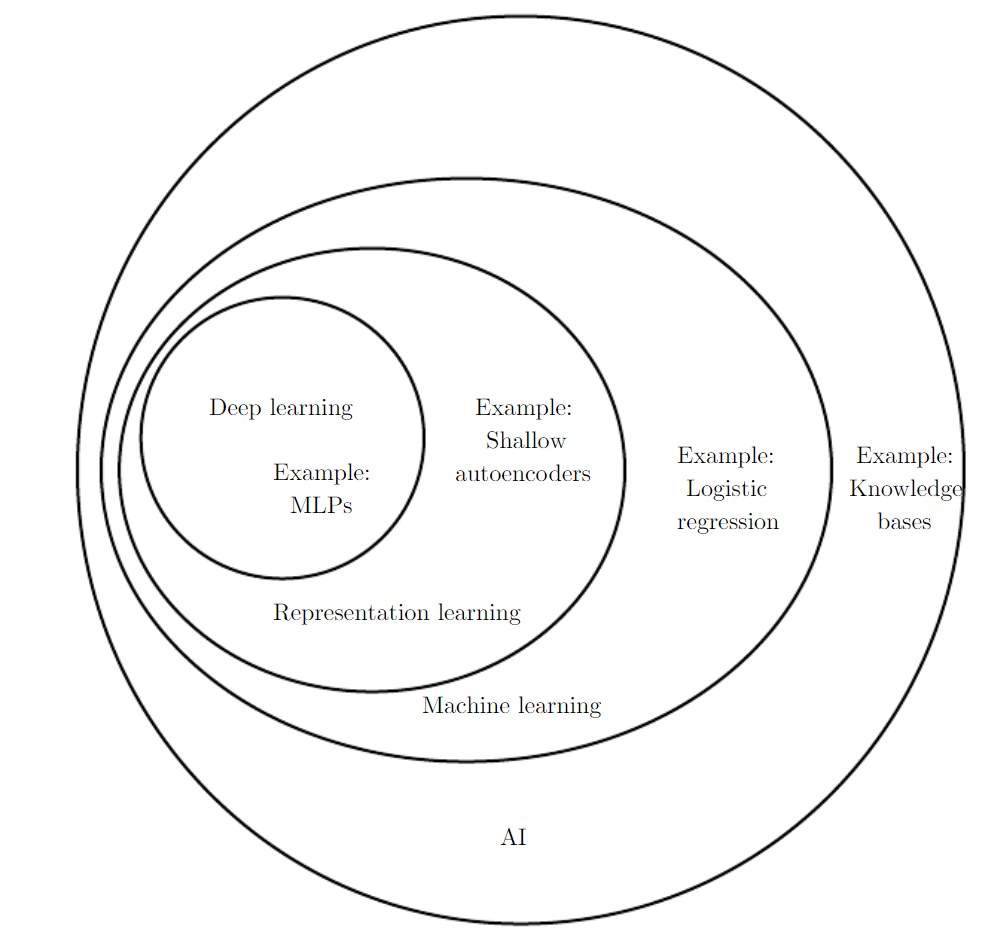
\includegraphics[scale=0.45]{images/venn_diagram_deeplearning.png}
    \centering
    \caption{Biểu đồ Venn về Trí tuệ nhân tạo}
    \label{fig:venn1}
\end{figure}


Một điểm đáng chú ý là học sâu cần một lượng lớn dữ liệu để huấn luyện mô hình một cách hiệu quả \cite{wiki-deep-learning}. Trong trường hợp OCR và nhận dạng hóa đơn, mạng nơron học sâu có khả năng học từ hàng nghìn hoặc thậm chí hàng triệu hình ảnh hóa đơn, điều này giúp mô hình hiểu rõ các đặc trưng và biểu diễn của dữ liệu hơn.

Hiện nay các kiến trúc học sâu như mạng nơ-ron sâu, mạng niềm tin sâu, học tăng cường sâu, mạng nơ-ron tái phát, mạng nơ-ron tích chập và máy biến áp đã được áp dụng cho các lĩnh vực bao gồm thị giác máy tính, nhận dạng giọng nói, xử lý ngôn ngữ tự nhiên, dịch máy, tin sinh học, thiết kế thuốc, Phân tích hình ảnh y tế, khoa học khí hậu, kiểm tra vật liệu và các chương trình trò chơi trên bàn cờ, nơi chúng đã tạo ra kết quả tương đương và trong một số trường hợp vượt qua hiệu suất chuyên gia của con người.

\subsubsection{Kiến trúc mạng nơ-ron nhân tạo}
Mạng nơ-ron nhân tạo là một mô hình được lấy cảm hứng từ mạng nơ-ron thần kinh. Kết hợp với các kĩ thuật học sâu, nó đang trở thành một công cụ rất mạnh mẽ mang lại hiệu quả tốt nhất cho nhiều bài toán khó như nhận dạng ảnh, giọng nói hay xử lý ngôn ngữ tự nhiên. Một mạng nơ-ron được cấu thành bởi các nơ-ron đơn lẻ được gọi là các perceptron.

Một perceptron sẽ nhận một hoặc nhiều đầu $\mathbf{x}$ vào dạng nhị phân và cho ra một kết quả $o$ dạng nhị phân duy nhất. Các đầu vào được điều phối tầm ảnh hưởng bởi các tham số trọng lượng tương ứng $\mathbf{w}$ của nó, còn kết quả đầu ra được quyết định dựa vào một ngưỡng quyết định $b$ nào đó:
$$o = \begin{cases}
        0 & \text{if } \sum_i w_i x_i +b \leq 0 \\
        1 & \text{if } \sum_i w_i x_i +b \ge 0
    \end{cases}$$

Mạng nơ-ron là sự kết hợp của của các tầng perceptron hay còn được gọi là perceptron đa tầng như hình vẽ bên dưới:
\begin{figure}[h]
    \begin{tikzpicture}[x=2.2cm,y=1.4cm]
    \message{^^JNeural network with arrows}
    \readlist\Nnod{4,5,5,5,3} % array of number of nodes per layer
    \message{^^J  Layer}
    \foreachitem \N \in \Nnod{ % loop over layers
        \edef\lay{\Ncnt} % alias of index of current layer
        \message{\lay,}
        \pgfmathsetmacro\prev{int(\Ncnt-1)} % number of previous layer
        \foreach \i [evaluate={\y=\N/2-\i; \x=\lay; \n=\nstyle;}] in {1,...,\N}{ % loop over nodes

                % NODES
                \node[node \n] (N\lay-\i) at (\x,\y) {$a_\i^{(\prev)}$};
                %\node[circle,inner sep=2] (N\lay-\i') at (\x-0.15,\y) {}; % shifted node
                %\draw[node] (N\lay-\i) circle (\R);

                % CONNECTIONS
                \ifnum\lay>1 % connect to previous layer
                    \foreach \j in {1,...,\Nnod[\prev]}{ % loop over nodes in previous layer
                            \draw[connect arrow] (N\prev-\j) -- (N\lay-\i); % connect arrows directly
                            %\draw[connect arrow] (N\prev-\j) -- (N\lay-\i'); % connect arrows to shifted node
                        }
                \fi % else: nothing to connect first layer
            }
    }
    % LABELS
    \node[above=5,align=center,mygreen!60!black] at (N1-1.90) {Lớp đầu vào};
    \node[above=2,align=center,myblue!60!black] at (N3-1.90) {Lớp ẩn};
    \node[above=8,align=center,myred!60!black] at (N\Nnodlen-1.90) {Lớp đầu ra};

\end{tikzpicture}
    \centering
    \caption{Kiến trúc một mạng Nơ-ron}

\end{figure}

Một mạng NN sẽ có 3 kiểu tầng \cite{aws-deep-learning}:
\begin{itemize}
    \item \textbf{Lớp đầu vào:} Một mạng nơ-ron nhân tạo sẽ có một số nút để nhập dữ liệu đầu vào. Các nút này tạo nên lớp đầu vào của hệ thống.
    \item \textbf{Lớp ẩn:} Lớp đầu vào xử lý và chuyển dữ liệu đến các lớp sâu hơn trong mạng nơ-ron. Các lớp ẩn này xử lý thông tin ở các cấp độ khác nhau, thích ứng với hành vi của mình khi nhận được thông tin mới. Các mạng học sâu có hàng trăm lớp ẩn có thể được dùng để phân tích một vấn đề từ nhiều góc độ khác nhau.
    \item \textbf{Lớp đầu ra:} Lớp đầu ra bao gồm các nút xuất dữ liệu. Các mô hình học sâu xuất ra đáp án "có" hoặc "không" chỉ có hai nút trong lớp đầu ra. Mặt khác, các mô hình xuất ra nhiều đáp án hơn sẽ có nhiều nút hơn.
\end{itemize}

Trong mạng Nơ-ron, mỗi nút mạng là một sigmoid nơ-ron nhưng hàm kích hoạt của chúng có thể khác nhau. Tuy nhiên trong thực tế người ta thường để chúng cùng dạng với nhau để tính toán cho thuận lợi.

Ở mỗi tầng, số lượng các nút mạng (nơ-ron) có thể khác nhau tuỳ thuộc vào bài toán và cách giải quyết. Nhưng thường khi làm việc người ta để các tầng ẩn có số lượng nơ-ron bằng nhau. Ngoài ra, các nơ-ron ở các tầng thường được liên kết đôi một với nhau tạo thành mạng kết nối đầy đủ. Khi đó ta có thể tính được kích cỡ của mạng dựa vào số tầng và số nơ-ron.

\subsubsection{Transformer}
Transformer là một kiến trúc mạng nơ-ron sâu được giới thiệu bởi Vaswani et al. trong bài báo "Attention Is All You Need \cite{vaswani2023attention}" vào năm 2017. Đây là một trong những tiến bộ quan trọng trong lĩnh vực xử lý ngôn ngữ tự nhiên và máy dịch dẫn đến những cải tiến đáng kể trong các ứng dụng như dịch máy, tổng hợp văn bản và nhiều nhiệm vụ khác liên quan đến ngôn ngữ.

Kiến trúc Transformer dựa trên cơ chế attention (sự chú ý), cho phép mạng có khả năng xem xét toàn bộ các phần của dữ liệu đầu vào cùng một lúc, thay vì như các kiến trúc trước đây phải đi qua từng bước theo thứ tự. Kiến trúc này có thể hoạt động với cả dữ liệu tuỳ chỉnh dài ngắn mà không cần giới hạn về chiều dài chuỗi đầu vào.

Transformer bao gồm hai phần chính: Encoder (Bộ mã hóa) và Decoder (Bộ giải mã). Cả hai phần đều sử dụng nhiều lớp "self-attention" (sự chú ý tự) để xác định sự quan hệ giữa các phần tử trong chuỗi đầu vào hoặc đầu ra. Sự chú ý tự cho phép mạng tập trung vào các phần tử quan trọng trong chuỗi và hiểu được mối quan hệ giữa chúng.

Transformer đã trở thành cơ sở cho nhiều kiến trúc mạng nơ-ron tiến tiến trong xử lý ngôn ngữ tự nhiên và thậm chí trong các ứng dụng khác như xử lý hình ảnh. Ví dụ nổi tiếng nhất có thể kể đến là "BERT" và "GPT" , cả hai đều là các biến thể của kiến trúc Transformer và đã đạt được những kết quả ấn tượng trong nhiều nhiệm vụ liên quan đến xử lý ngôn ngữ tự nhiên.

\paragraph{Kiến trúc Transformer}
Transformer tuân theo kiến trúc tổng thể này bằng cách sử dụng các lớp chú ý tự xếp chồng và các lớp kết nối đầy đủ theo điểm cho cả bộ mã hóa và bộ giải mã, như được thể hiện ở nửa trái và nửa phải của Hình \ref{fig3}. 
\begin{figure}[h]
    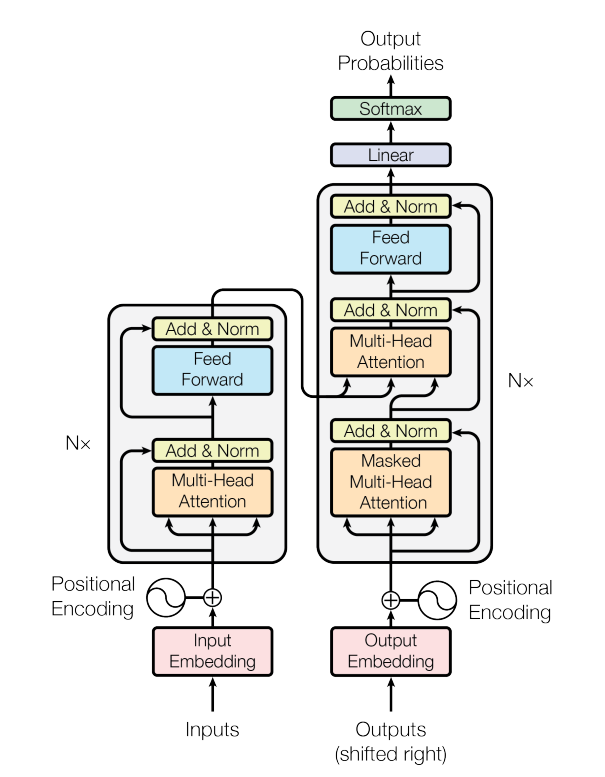
\includegraphics[scale=0.65]{images/transformer-architecture.png}
    \centering
    \caption{Kiến trúc tổng thể của Transformer \cite{vaswani2023attention}}
    \label{fig3}
\end{figure}

\paragraph{Ngăn xếp Encoder và Decoder}
\textbf{Bộ mã hóa}: Bộ giải mã có một ngăn xếp gồm $N = 6$ lớp identical. Mỗi lớp bao gồm hai lớp con. Lớp đầu tiên là cơ chế  multi-head self-attention, nơi mà mỗi từ trong câu đều "tương tác" với tất cả các từ khác để tạo ra sự chú ý chung trong ngữ cảnh. Lớp thứ hai là một mạng truyền thẳng kết nối đầy đủ theo từng vị trí, tức là thông tin từ mỗi vị trí trong câu được xử lý độc lập.

Để duy trì thông tin và hỗ trợ quá trình học, sử dụng kết nối residual xung quanh cả hai lớp con. Kết nối residual cho phép thông tin truyền từ đầu vào của lớp này đến đầu ra một cách dễ dàng. Sau đó, chúng ta thực hiện chuẩn hóa lớp để điều chỉnh phạm vi giá trị đầu ra. Cụ thể, đầu ra của mỗi lớp con được chuẩn hóa thông qua phép tính $\text{LayerNorm}(x + \text{Sublayer}(x))$, trong đó $\text{Sublayer}(x)$ là chức năng được thực hiện bởi chính lớp con đó.

Để đảm bảo tính nhất quán và khả năng kết nối residual, tất cả các lớp con trong mô hình cùng với các lớp nhúng đều tạo ra đầu ra với chiều $d_{model} = 512$, tức là có cùng kích thước đặc trưng để xử lý và truyền thông tin.

\textbf{Bộ giải mã}: Bộ giải mã cũng được tạo thành từ một ngăn xếp gồm $N = 6$ lớp identical. Bên cạnh hai lớp con trong mỗi lớp mã hóa, bộ giải mã thêm một lớp con thứ ba, thực hiện multi-head attention qua đầu ra của ngăn xếp bộ mã hóa. Tương tự như bộ mã hóa, chúng ta sử dụng kết nối residual xung quanh mỗi lớp con, sau đó là chuẩn hóa lớp. Điều chỉnh lớp con self-attention trong ngăn xếp bộ giải mã để ngăn các vị trí tập trung vào các vị trí tiếp theo. Thao tác này, kết hợp với việc lớp nhúng đầu ra được dịch chuyển một vị trí, đảm bảo rằng các dự đoán cho vị trí $i$ chỉ phụ thuộc vào đầu ra đã biết tại các vị trí nhỏ hơn $i$.

\paragraph{Attention}
Một hàm chú ý có thể được mô tả như việc ánh xạ một truy vấn và một tập hợp các cặp khóa-giá trị thành một đầu ra, trong đó truy vấn, khóa, giá trị và đầu ra đều là các vector. Đầu ra được tính toán dưới dạng tổng có trọng số của các giá trị, trong đó trọng số được gán cho mỗi giá trị được tính bằng một hàm tương thích của truy vấn với khóa tương ứng.

\paragraph{Scaled Dot-Product Attention}
Scaled Dot-Product Attention là một phần quan trọng của kiến trúc Transformer và cơ chế chú ý tự. Đầu vào của phương pháp này gồm các truy vấn (queries) và các khóa (keys) có kích thước $dk$, cùng với các giá trị (values) có kích thước $dv$. Tính tích vô hướng giữa truy vấn và tất cả các khóa, chia từng kết quả cho $dk$, sau đó áp dụng hàm softmax để thu được trọng số cho các giá trị. Thực hiện phép attention trên một tập hợp các truy vấn cùng lúc, gói chúng lại thành một ma trận $Q$. Các khóa và giá trị cũng được gói lại thành các ma trận $K$ và $V$. Kết quả đầu ra được tính bằng cách:
\[
    \text{Attention}(Q, K, V) = \text{softmax} (\frac{ QK^T }{ \sqrt{d_k} }) V   
\]

Bởi vì ảnh hưởng của tích vô hướng trở nên lớn về độ lớn, đẩy hàm softmax vào các vùng có độ dốc rất nhỏ.  Để chống lại tác động này,sử dụng tỷ lệ các tích vô hướng bằng \(\frac{1}{\sqrt{d_k}}\).

\paragraph{Multi-Head Attention}
Multi-Head Attention là một phần quan trọng trong kiến trúc Transformer. Trong chú ý đa đầu, một lớp chú ý thông thường được áp dụng nhiều lần với các trọng số khác nhau. Mỗi lần áp dụng này tạo ra một "Head Attention" riêng biệt. Mỗi Head Attention có thể tập trung vào các phần khác nhau của thông tin đầu vào và tạo ra các biểu diễn khác nhau. Sau đó, đầu ra của các Head Attention này được kết hợp để tạo ra đầu ra cuối cùng của chú ý Multi-Head.

Một tầng Multi-head Attention cho phép mô hình cùng lúc chú ý đến thông tin từ các không gian biểu diễn khác nhau tại các vị trí khác nhau. Với một attention head duy nhất, việc lấy trung bình ức chế khả năng này\cite{vaswani2023attention}.
\begin{align*}
    \text{MultiHead}(Q, K, V) &= \text{Concat}(\text{head}_1, \ldots, \text{head}_h)W^O \\
    \text{where head}_i &= \text{Attention}(QW_i^Q, KW_i^K, VW_i^V)
\end{align*}

Quá trình này giúp mô hình học cách tập trung vào các khía cạnh khác nhau của dữ liệu đầu vào và xử lý chúng một cách đa dạng. Chú ý đa đầu giúp kiến trúc Transformer hiệu quả hơn trong việc học các mối quan hệ và tương tác phức tạp trong dữ liệu ngôn ngữ và hình ảnh.

\subsubsection{Ứng dụng trong OCR}
Học sâu đã được chứng minh là có hiệu quả hơn các phương pháp OCR truyền thống \cite{ai-vs-traditional}, đặc biệt là đối với các tài liệu có chất lượng thấp hoặc bị định dạng phức tạp.

Một số ứng dụng của Học sâu trong OCR bao gồm:
\begin{itemize}
    \item Nhận dạng hóa đơn: Học sâu có thể được sử dụng để nhận dạng các trường thông tin quan trọng trên hóa đơn, chẳng hạn như tên người mua, người bán, ngày giao dịch, số lượng, giá và tổng số tiền. Điều này có thể giúp tiết kiệm thời gian và chi phí cho các doanh nghiệp, đồng thời cải thiện độ chính xác của việc xử lý hóa đơn.
    \item Nhận dạng tài liệu y tế: Học sâu có thể được sử dụng để nhận dạng thông tin quan trọng trên tài liệu y tế, chẳng hạn như tên bệnh nhân, chẩn đoán, phương pháp điều trị và các loại thuốc được kê đơn. Điều này có thể giúp cải thiện chất lượng chăm sóc bệnh nhân và giảm chi phí chăm sóc sức khỏe.
    \item Nhận dạng tài liệu pháp lý: Học sâu có thể được sử dụng để nhận dạng thông tin quan trọng trên tài liệu pháp lý, chẳng hạn như tên các bên liên quan, ngày tháng, các điều khoản của thỏa thuận và các điều khoản của hợp đồng. Điều này có thể giúp các luật sư và chuyên gia pháp lý tìm kiếm thông tin nhanh chóng và dễ dàng hơn.
    \item Nhận dạng tài liệu tài chính: Học sâu có thể được sử dụng để nhận dạng thông tin quan trọng trên tài liệu tài chính, chẳng hạn như tên công ty, giá cổ phiếu, số lượng cổ phiếu và giá trị thị trường của cổ phiếu. Điều này có thể giúp các nhà đầu tư và các chuyên gia tài chính đưa ra quyết định đầu tư tốt hơn.
\end{itemize}
Học sâu là một công nghệ mạnh mẽ có thể được sử dụng để cải thiện độ chính xác và hiệu quả của OCR. Với sự phát triển của Học sâu, OCR sẽ trở nên dễ dàng và thuận tiện hơn trong tương lai.

\subsection{Các thuật toán OCR}
Mặc dù OCR tương đối cụ thể, nhưng nó liên quan đến nhiều khía cạnh của công nghệ, bao gồm phát hiện văn bản, nhận dạng văn bản, nhận dạng văn bản từ đầu đến cuối, phân tích tài liệu, v.v. Nghiên cứu học thuật về các công nghệ liên quan của OCR phát triển mạnh mẽ. Phần này đây sẽ giới thiệu sơ lược về một số công nghệ chính trong tác vụ OCR.
\subsubsection{Phát hiện văn bản}
Công việc phát hiện văn bản là để xác định vùng chứa văn bản trên ảnh đầu vào. Trong những năm gần đây, có nhiều nghiên cứu học thuật về phát hiện văn bản. Một lớp phương pháp coi việc phát hiện văn bản như một tình huống cụ thể trong việc phát hiện mục tiêu, và điều chỉnh các thuật toán phát hiện mục tiêu chung để phù hợp với việc phát hiện văn bản. Ví dụ, TextBoxes dựa trên một bộ phát hiện mục tiêu một giai đoạn là SSD. Thuật toán điều chỉnh khung mục tiêu để vừa với các dòng văn bản có tỷ lệ khía cạnh cực đoan, trong khi CTPN được phát triển từ Faster RCNN. Tuy nhiên, vẫn có một số khác biệt giữa phát hiện văn bản và phát hiện mục tiêu về thông tin mục tiêu và nhiệm vụ chính. Ví dụ, văn bản thường dài và trông giống "vạch", khoảng cách giữa các dòng nhỏ, văn bản có thể uốn cong, v.v. Do đó, nhiều thuật toán đặc biệt cho việc phát hiện văn bản đã được phát triển, như EAST, PSENet, DBNet, và nhiều thuật toán khác \cite{Dive-into-ocr-2022}.
\begin{figure}
    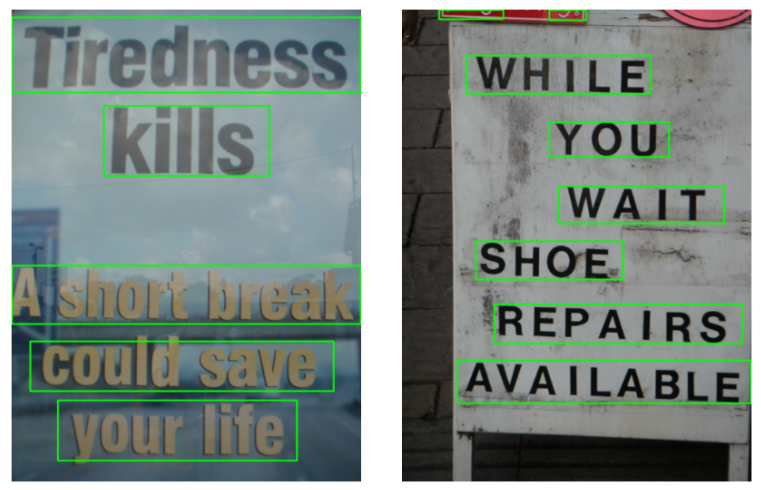
\includegraphics[scale=0.7]{images/text-detection.png}
    \centering
    \caption{Ví dụ về nhiệm vụ phát hiện văn bản}
\end{figure}

Hiện tại, một số thuật toán phát hiện văn bản phổ biến có thể được chia ra một cách đại khái thành hai loại: \textbf{Thuật toán dựa trên Hồi quy} và \textbf{Thuật toán dựa trên Phân đoạn}. Cũng có một số thuật toán kết hợp cả hai loại này. Các thuật toán dựa trên hồi quy lấy cảm hứng từ các thuật toán phát hiện đối tượng chung, thực hiện việc hồi quy hộp phát hiện bằng cách đặt các anchor, hoặc thậm chí trực tiếp thực hiện hồi quy điểm ảnh. Loại phương pháp này hoạt động tốt trong việc phân biệt văn bản có hình dạng đều đặn, nhưng kém trong việc phát hiện văn bản có hình dạng không đều. Ví dụ, CTPN tốt trong việc nhận dạng văn bản ngang, nhưng kém trong việc phát hiện văn bản uốn cong và xoắn. SegLink phù hợp hơn với văn bản dài, nhưng không thích hợp cho việc phát hiện văn bản phân tán thưa thớt. Các thuật toán dựa trên phân đoạn giới thiệu Mask-RCNN, loại thuật toán này có thể hoạt động tốt hơn trong việc phát hiện trong các tình huống và văn bản có các hình dạng khác nhau, nhưng hạn chế là việc xử lý sau cùng phức tạp, vì vậy có thể chậm về tốc độ và không thể phát hiện được văn bản chồng lấn \cite{Dive-into-ocr-2022}.

\begin{figure}[h]
    \tikzset{every picture/.style={line width=0.75pt}} %set default line width to 0.75pt        
\begin{tikzpicture}[x=0.75pt,y=0.75pt,yscale=-1,xscale=1]
    %uncomment if require: \path (0,783); %set diagram left start at 0, and has height of 783

    %Rounded Rect [id:dp12536916830339373] 
    \draw  [color={rgb, 255:red, 246; green, 35; blue, 35 }  ,draw opacity=1 ][fill={rgb, 255:red, 246; green, 35; blue, 35 }  ,fill opacity=1 ] (79.8,126.47) .. controls (79.8,120.47) and (84.67,115.6) .. (90.67,115.6) -- (238.49,115.6) .. controls (244.5,115.6) and (249.37,120.47) .. (249.37,126.47) -- (249.37,159.1) .. controls (249.37,165.1) and (244.5,169.97) .. (238.49,169.97) -- (90.67,169.97) .. controls (84.67,169.97) and (79.8,165.1) .. (79.8,159.1) -- cycle ;
    %Straight Lines [id:da35079927471568495] 
    \draw    (484.18,93.97) -- (484.52,110.57) ;
    \draw [shift={(484.58,113.57)}, rotate = 268.83] [fill={rgb, 255:red, 0; green, 0; blue, 0 }  ][line width=0.08]  [draw opacity=0] (8.93,-4.29) -- (0,0) -- (8.93,4.29) -- cycle    ;
    %Straight Lines [id:da3515453488418392] 
    \draw    (484.18,93.97) -- (164.67,93.67) ;
    %Straight Lines [id:da8167979499170375] 
    \draw    (164.67,93.67) -- (164.67,111.07) ;
    \draw [shift={(164.67,114.07)}, rotate = 270] [fill={rgb, 255:red, 0; green, 0; blue, 0 }  ][line width=0.08]  [draw opacity=0] (8.93,-4.29) -- (0,0) -- (8.93,4.29) -- cycle    ;
    %Straight Lines [id:da24241956645024332] 
    \draw    (324.61,75.97) -- (324.42,93.82) ;
    %Rounded Rect [id:dp4800123674594827] 
    \draw  [color={rgb, 255:red, 0; green, 33; blue, 205 }  ,draw opacity=1 ][fill={rgb, 255:red, 0; green, 33; blue, 205 }  ,fill opacity=1 ] (399.8,125.67) .. controls (399.8,119.67) and (404.67,114.8) .. (410.67,114.8) -- (558.49,114.8) .. controls (564.5,114.8) and (569.37,119.67) .. (569.37,125.67) -- (569.37,158.3) .. controls (569.37,164.3) and (564.5,169.17) .. (558.49,169.17) -- (410.67,169.17) .. controls (404.67,169.17) and (399.8,164.3) .. (399.8,158.3) -- cycle ;
    %Rounded Rect [id:dp7078369789993373] 
    \draw  [color={rgb, 255:red, 36; green, 159; blue, 255 }  ,draw opacity=1 ][fill={rgb, 255:red, 255; green, 255; blue, 255 }  ,fill opacity=0 ] (242.2,31.67) .. controls (242.2,25.67) and (247.07,20.8) .. (253.07,20.8) -- (400.89,20.8) .. controls (406.9,20.8) and (411.77,25.67) .. (411.77,31.67) -- (411.77,64.3) .. controls (411.77,70.3) and (406.9,75.17) .. (400.89,75.17) -- (253.07,75.17) .. controls (247.07,75.17) and (242.2,70.3) .. (242.2,64.3) -- cycle ;
    %Rounded Rect [id:dp5367367596794104] 
    \draw  [fill={rgb, 255:red, 255; green, 255; blue, 255 }  ,fill opacity=0 ][dash pattern={on 4.5pt off 4.5pt}] (22.33,240.83) .. controls (22.33,209.04) and (48.1,183.27) .. (79.89,183.27) -- (252.57,183.27) .. controls (284.36,183.27) and (310.13,209.04) .. (310.13,240.83) -- (310.13,489.65) .. controls (310.13,521.44) and (284.36,547.21) .. (252.57,547.21) -- (79.89,547.21) .. controls (48.1,547.21) and (22.33,521.44) .. (22.33,489.65) -- cycle ;
    %Rounded Rect [id:dp2663541401208218] 
    \draw  [fill={rgb, 255:red, 255; green, 255; blue, 255 }  ,fill opacity=0 ][dash pattern={on 4.5pt off 4.5pt}] (342.33,237.83) .. controls (342.33,206.04) and (368.1,180.27) .. (399.89,180.27) -- (572.57,180.27) .. controls (604.36,180.27) and (630.13,206.04) .. (630.13,237.83) -- (630.13,486.65) .. controls (630.13,518.44) and (604.36,544.21) .. (572.57,544.21) -- (399.89,544.21) .. controls (368.1,544.21) and (342.33,518.44) .. (342.33,486.65) -- cycle ;


    % Text Node
    \draw (42,364.54) node [anchor=north west][inner sep=0.75pt]   [align=left] {\textcolor[rgb]{0,0.09,0.75}{Ưu: Thường tốt cho văn bản }\\\textcolor[rgb]{0,0.09,0.75}{hình dạng thông thường.}\\\textcolor[rgb]{0,0.09,0.75}{Nhược: \ Không được chính xác}\\\textcolor[rgb]{0,0.09,0.75}{khi phát hiện văn bản có hình dạng}\\\textcolor[rgb]{0,0.09,0.75}{ bất thường}};
    % Text Node
    \draw (282.8,46.8) node [anchor=north west][inner sep=0.75pt]   [align=left] {{\small \textbf{phát hiện}}};
    % Text Node
    \draw (270.85,32.97) node [anchor=north west][inner sep=0.75pt]   [align=left] {{\small \textbf{Các thuật toán}}};
    % Text Node
    \draw (104.35,135.57) node [anchor=north west][inner sep=0.75pt]   [align=left] {{\small \textcolor[rgb]{1,1,1}{Dựa trên hồi quy}}};
    % Text Node
    \draw (423.47,135.37) node [anchor=north west][inner sep=0.75pt]   [align=left] {{\small \textcolor[rgb]{1,1,1}{Dựa trên phân vùng}}};
    % Text Node
    \draw (84,208.33) node [anchor=north west][inner sep=0.75pt]   [align=left] {CTPN\\Textboxes/Texboxes++\\EAST\\CRAFT\\...};
    % Text Node
    \draw (404,207.67) node [anchor=north west][inner sep=0.75pt]   [align=left] {Pixel embeding\\PSENet\\PAN\\DB/DB++\\...};
    % Text Node
    \draw (363,361.54) node [anchor=north west][inner sep=0.75pt]   [align=left] {\textcolor[rgb]{0,0.09,0.75}{Ưu: Xử lý tốt với văn bản có hình }\\\textcolor[rgb]{0,0.09,0.75}{dạng khác nhau.}\\\textcolor[rgb]{0,0.09,0.75}{Nhược: \ Quá trình hậu xử lý phức}\\\textcolor[rgb]{0,0.09,0.75}{tạp, tốn thời gian và hiệu quả kém}\\\textcolor[rgb]{0,0.09,0.75}{với văn bản chồng chéo}};
\end{tikzpicture}
    \centering
    \caption{Tổng quan về thuật toán phát hiện văn bản}
\end{figure}
\subsubsection{Nhận dạng văn bản}
Nhận dạng văn bản là việc nhận biết nội dung văn bản trong hình ảnh, và đầu vào thường là từ phần vùng chứa văn bản của ảnh được cắt ra bằng hộp văn bản được tạo ra từ việc phát hiện văn bản. Nhận dạng văn bản có thể được chia thành hai loại chính: \textbf{Nhận dạng Văn bản Đều đặn} và \textbf{Nhận dạng Văn bản Không đều đặn} dựa trên đường viền của văn bản cần nhận dạng.

\begin{figure}[h]
    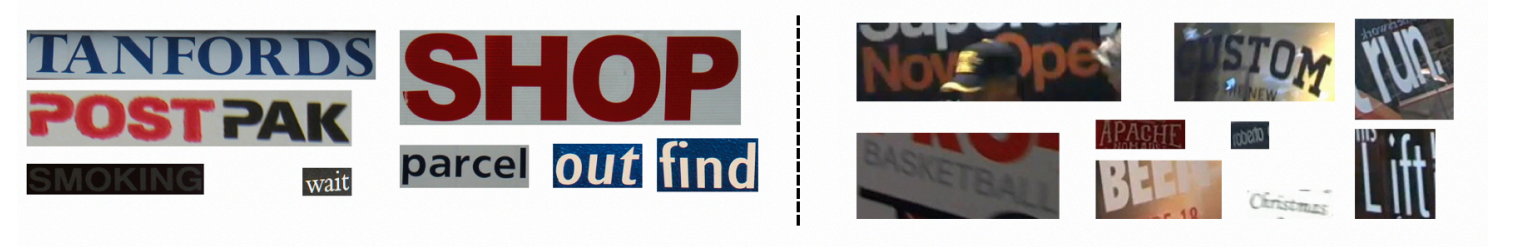
\includegraphics[scale=0.4]{images/regular-irregular-text.png}
    \centering
    \caption{Văn bản đều đặn (trái) và Văn bản không đều đặn (phải)}
\end{figure}

Văn bản đều đặn chủ yếu đề cập đến các phông chữ in, văn bản được quét, và các nguồn tương tự có hướng chính đều. Văn bản không đều đặn thường không nằm trong tư thế ngang, thường uốn cong, bị che khuất và mờ mờ. Các tình huống văn bản không đều đặn thách thức rất lớn, và đó cũng là hướng nghiên cứu chính trong việc nhận dạng văn bản.

Các thuật toán nhận dạng văn bản đều đặn có thể được chia thành hai loại dựa trên các phương pháp giải mã khác nhau: Thuật toán dựa trên CTC và Thuật toán dựa trên Sequence2Sequence. Chúng khác nhau trong cách chuyển đổi các đặc trưng chuỗi mà mạng học học được thành kết quả nhận dạng cuối cùng. Một ví dụ đại diện cho thuật toán dựa trên CTC là CRNN cổ điển.

\begin{figure}[p]
    \tikzset{every picture/.style={line width=0.75pt}} %set default line width to 0.75pt        

\begin{tikzpicture}[x=0.75pt,y=0.75pt,yscale=-1,xscale=1]
    %uncomment if require: \path (0,819); %set diagram left start at 0, and has height of 819

    %Rounded Rect [id:dp7357497005786489] 
    \draw  [dash pattern={on 4.5pt off 4.5pt}] (78.38,111.44) .. controls (78.38,78.6) and (105,51.98) .. (137.84,51.98) -- (484.66,51.98) .. controls (517.5,51.98) and (544.12,78.6) .. (544.12,111.44) -- (544.12,289.82) .. controls (544.12,322.66) and (517.5,349.28) .. (484.66,349.28) -- (137.84,349.28) .. controls (105,349.28) and (78.38,322.66) .. (78.38,289.82) -- cycle ;
    %Up Down Arrow [id:dp10182102951041139] 
    \draw  [color={rgb, 255:red, 0; green, 0; blue, 0 }  ,draw opacity=0 ][fill={rgb, 255:red, 255; green, 0; blue, 0 }  ,fill opacity=1 ] (206.27,365.77) -- (220.2,357.52) -- (234.13,365.77) -- (227.16,365.77) -- (227.16,382.27) -- (234.13,382.27) -- (220.2,390.52) -- (206.27,382.27) -- (213.23,382.27) -- (213.23,365.77) -- cycle ;
    %Up Down Arrow [id:dp6666173009893719] 
    \draw  [color={rgb, 255:red, 0; green, 0; blue, 0 }  ,draw opacity=0 ][fill={rgb, 255:red, 255; green, 0; blue, 0 }  ,fill opacity=1 ] (406.67,365.77) -- (420.6,357.52) -- (434.53,365.77) -- (427.56,365.77) -- (427.56,382.27) -- (434.53,382.27) -- (420.6,390.52) -- (406.67,382.27) -- (413.63,382.27) -- (413.63,365.77) -- cycle ;
    %Rounded Rect [id:dp06853301880737295] 
    \draw  [dash pattern={on 4.5pt off 4.5pt}] (77.38,457.44) .. controls (77.38,424.6) and (104,397.98) .. (136.84,397.98) -- (483.66,397.98) .. controls (516.5,397.98) and (543.12,424.6) .. (543.12,457.44) -- (543.12,635.82) .. controls (543.12,668.66) and (516.5,695.28) .. (483.66,695.28) -- (136.84,695.28) .. controls (104,695.28) and (77.38,668.66) .. (77.38,635.82) -- cycle ;

    % Text Node
    \draw (222,465.41) node   [align=left] {\begin{minipage}[lt]{68pt}\setlength\topsep{0pt}
            CRNN\\STAR-Net\\Rosetta\\...
        \end{minipage}};
    % Text Node
    \draw (407,465.91) node   [align=left] {\begin{minipage}[lt]{68pt}\setlength\topsep{0pt}
            R2AM\\SAR\\RARE\\...
        \end{minipage}};
    % Text Node
    \draw (209.63,593.06) node   [align=left] {\begin{minipage}[lt]{134.82pt}\setlength\topsep{0pt}
            \textcolor[rgb]{0,0.45,0.08}{Ưu: Hiệu quả cao, tốt cho văn bản thông thường và dài}\\\textcolor[rgb]{1,0,0}{Nhược: Không sử dụng thông tin ngữ cảnh}
        \end{minipage}};
    % Text Node
    \draw (419.63,581.49) node   [align=left] {\begin{minipage}[lt]{134.82pt}\setlength\topsep{0pt}
            \textcolor[rgb]{0,0.45,0.08}{Ưu: Độ chính xác cao}\\\textcolor[rgb]{1,0,0}{Nhược: Hiệu quả kém cho văn bản quá dài hoặc quá ngắn}
        \end{minipage}};
    % Text Node
    \draw  [color={rgb, 255:red, 74; green, 144; blue, 226 }  ,draw opacity=1 ]  (247.07,78.7) .. controls (247.07,69.86) and (254.24,62.7) .. (263.07,62.7) -- (346.07,62.7) .. controls (354.91,62.7) and (362.07,69.86) .. (362.07,78.7) -- (362.07,92.7) .. controls (362.07,101.53) and (354.91,108.7) .. (346.07,108.7) -- (263.07,108.7) .. controls (254.24,108.7) and (247.07,101.53) .. (247.07,92.7) -- cycle  ;
    \draw (304.57,85.7) node   [align=left] {\begin{minipage}[lt]{75.58pt}\setlength\topsep{0pt}
            \begin{center}
                Thuật toán nhận dạng
            \end{center}

        \end{minipage}};
    % Text Node
    \draw  [color={rgb, 255:red, 0; green, 0; blue, 0 }  ,draw opacity=0 ][fill={rgb, 255:red, 145; green, 9; blue, 181 }  ,fill opacity=1 ]  (158.74,151.2) .. controls (158.74,142.37) and (165.9,135.2) .. (174.74,135.2) -- (257.74,135.2) .. controls (266.58,135.2) and (273.74,142.37) .. (273.74,151.2) -- (273.74,167.2) .. controls (273.74,176.04) and (266.58,183.2) .. (257.74,183.2) -- (174.74,183.2) .. controls (165.9,183.2) and (158.74,176.04) .. (158.74,167.2) -- cycle  ;
    \draw (216.24,159.2) node  [color={rgb, 255:red, 255; green, 255; blue, 255 }  ,opacity=1 ] [align=left] {\begin{minipage}[lt]{75.58pt}\setlength\topsep{0pt}
            \begin{center}
                CTC-based
            \end{center}

        \end{minipage}};
    % Text Node
    \draw  [color={rgb, 255:red, 0; green, 0; blue, 0 }  ,draw opacity=0 ][fill={rgb, 255:red, 0; green, 81; blue, 33 }  ,fill opacity=1 ]  (347.41,152.04) .. controls (347.41,143.2) and (354.57,136.04) .. (363.41,136.04) -- (446.41,136.04) .. controls (455.24,136.04) and (462.41,143.2) .. (462.41,152.04) -- (462.41,166.04) .. controls (462.41,174.88) and (455.24,182.04) .. (446.41,182.04) -- (363.41,182.04) .. controls (354.57,182.04) and (347.41,174.88) .. (347.41,166.04) -- cycle  ;
    \draw (404.91,159.04) node  [color={rgb, 255:red, 255; green, 255; blue, 255 }  ,opacity=1 ] [align=left] {\begin{minipage}[lt]{75.58pt}\setlength\topsep{0pt}
            \begin{center}
                Attention-based
            \end{center}

        \end{minipage}};
    % Text Node
    \draw (146.33,205.31) node [anchor=north west][inner sep=0.75pt]   [align=left] {\mbox{-} CRNN+CTC\\\mbox{-} Giới thiệu một ký tự không \\gian\\\mbox{-} Nhãn không yêu cầu căn \\chỉnh cấp độ ký tự};
    % Text Node
    \draw (337,206.33) node [anchor=north west][inner sep=0.75pt]   [align=left] {\mbox{-} Seq2Seq+attention};
    % Connection
    \draw    (276.93,108.7) -- (246.62,133.92) ;
    \draw [shift={(245.08,135.2)}, rotate = 320.24] [color={rgb, 255:red, 0; green, 0; blue, 0 }  ][line width=0.75]    (10.93,-3.29) .. controls (6.95,-1.4) and (3.31,-0.3) .. (0,0) .. controls (3.31,0.3) and (6.95,1.4) .. (10.93,3.29)   ;
    % Connection
    \draw    (336.04,108.7) -- (371.83,134.86) ;
    \draw [shift={(373.44,136.04)}, rotate = 216.17] [color={rgb, 255:red, 0; green, 0; blue, 0 }  ][line width=0.75]    (10.93,-3.29) .. controls (6.95,-1.4) and (3.31,-0.3) .. (0,0) .. controls (3.31,0.3) and (6.95,1.4) .. (10.93,3.29)   ;

\end{tikzpicture}
    \centering
    \caption{CTC-based recognition algorithm VS. Attention-based recognition algorithm}
\end{figure}

Các thuật toán nhận dạng cho văn bản không đều đặn phong phú hơn. Các phương pháp như STAR-Net sửa chữa đường viền của văn bản không đều đặn thành các hình chữ nhật đều đặn bằng cách thêm các mô-đun sửa chữa như TPS trước khi thực hiện việc nhận dạng. Các phương pháp dựa trên Attention như RARE chú trọng hơn đến mối quan hệ giữa các phần trong chuỗi. Các phương pháp dựa trên phân đoạn xử lý mỗi ký tự trên dòng văn bản như một đơn vị riêng lẻ, làm cho việc nhận dạng ký tự đã phân đoạn dễ dàng hơn so với việc nhận dạng toàn bộ dòng văn bản sau khi sửa chữa. Ngoài ra, với sự phát triển nhanh chóng của Transformer và hiệu quả đã được xác minh trong các nhiệm vụ khác nhau trong những năm gần đây, nhiều thuật toán nhận dạng văn bản dựa trên transformer đã phát triển mạnh mẽ. Loại giải pháp này sử dụng cấu trúc transformer để giải quyết việc mô hình hóa sự phụ thuộc lâu dài trong CNN và đã đạt được kết quả tốt.

\begin{figure}
    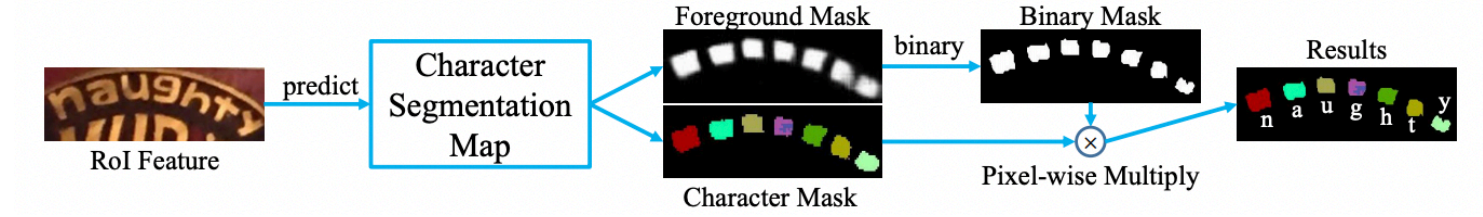
\includegraphics[scale=0.40]{images/recognition-based-charcter-segmentation.png}
    \centering
    \caption{Thuật toán nhận dạng dựa trên phân vùng ký tự}
\end{figure}

\subsubsection{Nhận dạng cấu trúc tài liệu}
Công nghệ OCR có thể đáp ứng yêu cầu về phát hiện và nhận dạng văn bản. Tuy nhiên, trong các tình huống thực tế, điều chúng ta thường cần là thông tin có cấu trúc, chẳng hạn như trích xuất thông tin từ thẻ ID và hóa đơn, xác định có cấu trúc của bảng, và vân vân. Các tình huống ứng dụng của công nghệ OCR chủ yếu là trích xuất tài liệu nhanh, so sánh nội dung hợp đồng, so sánh thông tin tài chính trên các tài liệu cần thanh toán, và xác định tài liệu vận chuyển. Kết quả OCR + xử lý sau cùng là một kế hoạch cấu trúc thường được sử dụng, nhưng phức tạp và cần thiết phải được thiết kế cẩn thận, và thiếu sự tổng quát. Với sự phát triển liên tục của công nghệ OCR và nhu cầu về trích xuất thông tin có cấu trúc đang gia tăng, các công nghệ liên quan đến phân tích tài liệu thông minh, như phân tích bố cục, nhận dạng bảng, và trích xuất thông tin quan trọng, đã nhận được sự chú ý ngày càng tăng.

\paragraph{Phân tích bố cục}
Phân tích bố cục được thực hiện để phân loại nội dung của hình ảnh tài liệu thành các loại như văn bản thuần túy, tiêu đề, bảng biểu, hình ảnh, v.v. Các phương pháp hiện tại thường thực hiện việc phát hiện hoặc phân đoạn chúng một cách riêng biệt. Ví dụ, Soto Carlos sử dụng thông tin ngữ cảnh và vị trí tự nhiên của nội dung tài liệu để cải thiện hiệu suất phát hiện vùng dựa trên thuật toán phát hiện mục tiêu Faster R-CNN. Sarkar Mausoom và đồng nghiệp đề xuất một cơ chế phân đoạn dựa trên tiên biết để huấn luyện mô hình phân đoạn tài liệu với các hình ảnh có độ phân giải cao, giải quyết vấn đề rằng các cấu trúc khác nhau trong các khu vực dày đặc không thể phân biệt và hợp nhất do việc giảm quá mức của hình ảnh gốc.

\paragraph{Nhận dạng bảng}
Nhận dạng bảng là việc xác định và chuyển thông tin bảng của tài liệu thành một tệp Excel. Có nhiều loại và phong cách bảng khác nhau trong hình ảnh văn bản, chẳng hạn như các hàng và cột khác nhau và các loại văn bản khác nhau. Ngoài ra, phong cách của tài liệu và môi trường ánh sáng khi chụp ảnh đã đặt ra những thách thức lớn cho việc nhận dạng bảng, làm cho việc nhận dạng bảng trở thành một vấn đề nghiên cứu khó khăn trong việc hiểu tài liệu. Có nhiều phương pháp nhận dạng bảng. Ví dụ, vào những ngày đầu tiên, có các thuật toán truyền thống dựa trên các quy tắc heuristics, như thuật toán T-Rect được đề xuất bởi Kieninger và cộng sự, thường sử dụng quy tắc thiết kế thủ công và phát hiện và phân tích miền kết nối. Trong những năm gần đây, khi học sâu tiếp tục phát triển, một số thuật toán nhận dạng cấu trúc bảng dựa trên mạng CNN đã xuất hiện, như DeepTabStR được đề xuất bởi Siddiqui Shoaib Ahmed và cộng sự và TabStruct-Net được đề xuất bởi Raja Sachin và cộng sự. Ngoài ra, với sự gia tăng của Mạng Neural Đồ thị, một số nhà nghiên cứu đã thử áp dụng Mạng Neural Đồ thị vào việc nhận dạng cấu trúc bảng và coi việc nhận dạng bảng như một vấn đề tái tạo đồ thị dựa trên Mạng Neural Đồ thị. Đây là cách mà TGRNet được đề xuất bởi Xue Wenyuan và cộng sự hoạt động. Hơn nữa, có các giải pháp end-to-end có kết quả đầu ra cấu trúc bảng dưới dạng HTML bằng mạng. Hầu hết trong số này áp dụng Seq2Seq để dự đoán cấu trúc bảng như những thuật toán dựa trên attention hoặc transformer, bao gồm TableMaster.

\paragraph{Trích xuất thông tin chính}
Trích xuất thông tin quan trọng (KIE) là một nhiệm vụ quan trọng trong Hỏi và Trả lời Văn bản (Document VQA). Nó liên quan đến việc trích xuất thông tin cần thiết từ hình ảnh, chẳng hạn như tên và số ID từ thẻ ID. Thông tin như vậy thường được xác định trong một nhiệm vụ, nhưng khác nhau giữa các nhiệm vụ khác nhau.

\begin{figure}[h!]
    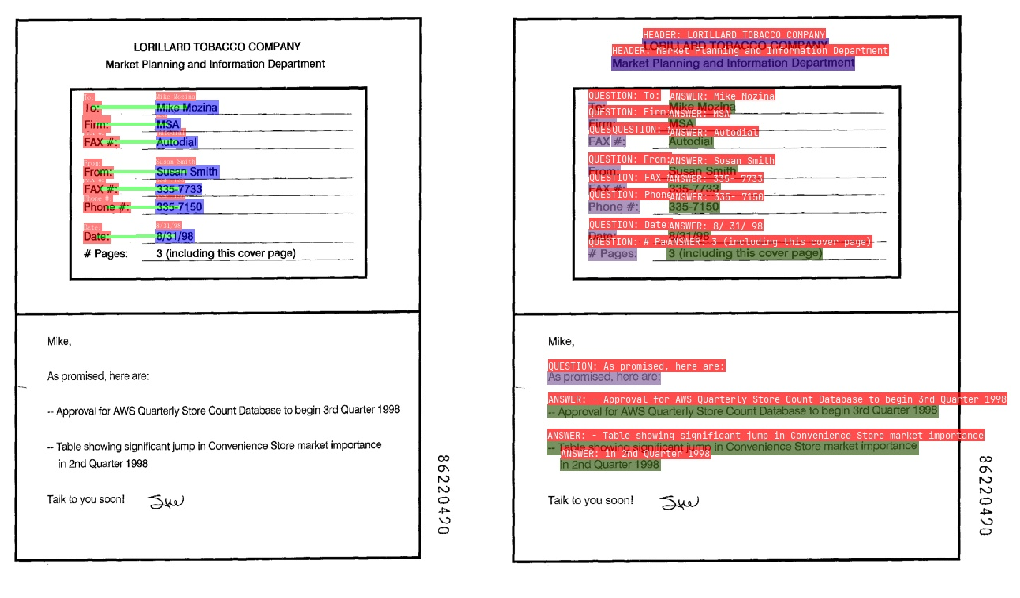
\includegraphics[scale=0.6]{images/re-vs-ser.png}
    \centering
    \caption{RE(trái) VS SER(phải)}
    \label{fig8:ser-re}
\end{figure}

KIE thường được chia thành hai phần nhiệm vụ con để nghiên cứu (Hình \ref{fig8:ser-re}):
\begin{itemize}
    \item SER: Đây là việc nhận dạng thực thể ngữ nghĩa, phân loại từng đoạn văn bản được phát hiện. Ví dụ, nó chia văn bản thành tên và số thẻ ID như hình dưới đây.
    \item RE: Đây là việc trích xuất mối quan hệ, phân loại từng đoạn văn bản. Ví dụ, nó có thể phân loại văn bản thành câu hỏi và câu trả lời, sau đó tìm câu trả lời tương ứng cho mỗi câu hỏi. Như hình dưới đây, các hộp đỏ và đen đại diện cho câu hỏi và câu trả lời tương ứng, và các mũi tên màu vàng chỉ sự tương ứng giữa câu hỏi và câu trả lời.
\end{itemize}
Phương pháp KIE thông thường được phát triển dựa trên nhận dạng thực thể đặt tên (NER), nhưng loại phương pháp này chỉ sử dụng thông tin văn bản trong hình ảnh mà không sử dụng thông tin hình ảnh và cấu trúc. Do đó, nó không đạt độ chính xác cao. Trong những năm gần đây, nhiều giải pháp đã bắt đầu kết hợp thông tin hình ảnh và cấu trúc với thông tin văn bản. Do sử dụng các nguyên tắc khác nhau trong việc kết hợp thông tin đa tầng, các phương pháp này có thể được chia thành bốn loại:
\begin{itemize}
    \item Phương pháp dựa trên lưới
    \item Phương pháp dựa trên token
    \item Phương pháp dựa trên Graph Convolutional Network
    \item Phương pháp end-to-end
\end{itemize}